% --- Foundation Models vs. Large Language Models (LLMs): Overview ---
% % Figures from Bommasani et al., arXiv:2108.07258 (Stanford CRFM).
% \begin{frame}{Foundation Models vs. LLMs: Overview}
%   \begin{itemize}
%     \item \textbf{Definition:} A \emph{foundation model} is trained on \textbf{broad and diverse data} (often with \textbf{self-supervision} at scale) to learn universal representations, and can then be \textbf{adapted} (through fine-tuning, prompting, etc.) to a wide range of downstream tasks and modalities. Rather than being built for a single end-task, the same pretrained backbone can be specialized for applications such as QA, captioning, recognition, and more across different domains.
%     \item \textbf{LLMs:} Text-centric foundation models (e.g.\ BERT, GPT) whose pretraining is dominated by language modeling; many multimodal systems today \emph{add} vision or audio encoders on top of an LLM.
%     \item \textcolor{KAUSTred}{\bf Key point:} \textit{LLMs are foundation models for language; not every foundation model is an LLM.}
%   \end{itemize}
%   \vspace{0.15cm}
% \end{frame}

% --- Foundation models vs.\ LLMs and ecosystem implications ---
% --- Key Differences: Modalities, Tasks, and Architecture ---
\begin{frame}{Key Differences: Modalities, Tasks, and Adaptation}
  \begin{columns}[T,onlytextwidth]
    \begin{column}{0.48\textwidth}
      \textbf{Foundation models}
      \begin{itemize}\footnotesize
        \item Trained on \textbf{heterogeneous} data: text, images, speech, structured data, 3D/signals, \ldots\ (see Fig.~2).
        \item \textbf{Homogenization:} one pretrained model is adapted to many applications; \textbf{emergence:} capabilities (e.g.\ in-context learning) from scale were not explicitly programmed.
        \item Objectives: self-supervised / contrastive / masked / alignment---not only next-token prediction.
      \end{itemize}
    \end{column}
    \begin{column}{0.48\textwidth}
      \textbf{LLMs}
      \begin{itemize}\footnotesize
        \item \textbf{Language-first:} data are primarily text; core loss is usually autoregressive or masked LM.
        \item \textbf{Downstream:} generation, QA, summarization, code; multimodal \textbf{variants} pair an LLM with other encoders.
        \item Same ``pretrain then adapt'' pattern, but the \textbf{scope of pretraining data} is narrower than full multi-modal foundation models.
      \end{itemize}
    \end{column}
  \end{columns}
  \vspace{0.2cm}
\end{frame}

% --- Implications: Use Cases and Limitations ---
\begin{frame}{Implications: Ecosystem and Deployment}
  \begin{itemize}\footnotesize
    \item \textbf{Foundation models} enable transfer across domains (vision--language, robotics, biomedicine, \ldots) but concentrate capability in a few shared pretrained artifacts.
    \item \textbf{LLMs} excel at language and code; for vision, video, or tabular data they are usually \textbf{one component} of a larger system unless trained multi-modally from the start.
    \item \textbf{Limitations:} compute and data scale, inherited biases from pretraining, evaluation and safety gaps as the same ``foundation'' is reused widely.
  \end{itemize}
  \vspace{0.15cm}
  \centering
  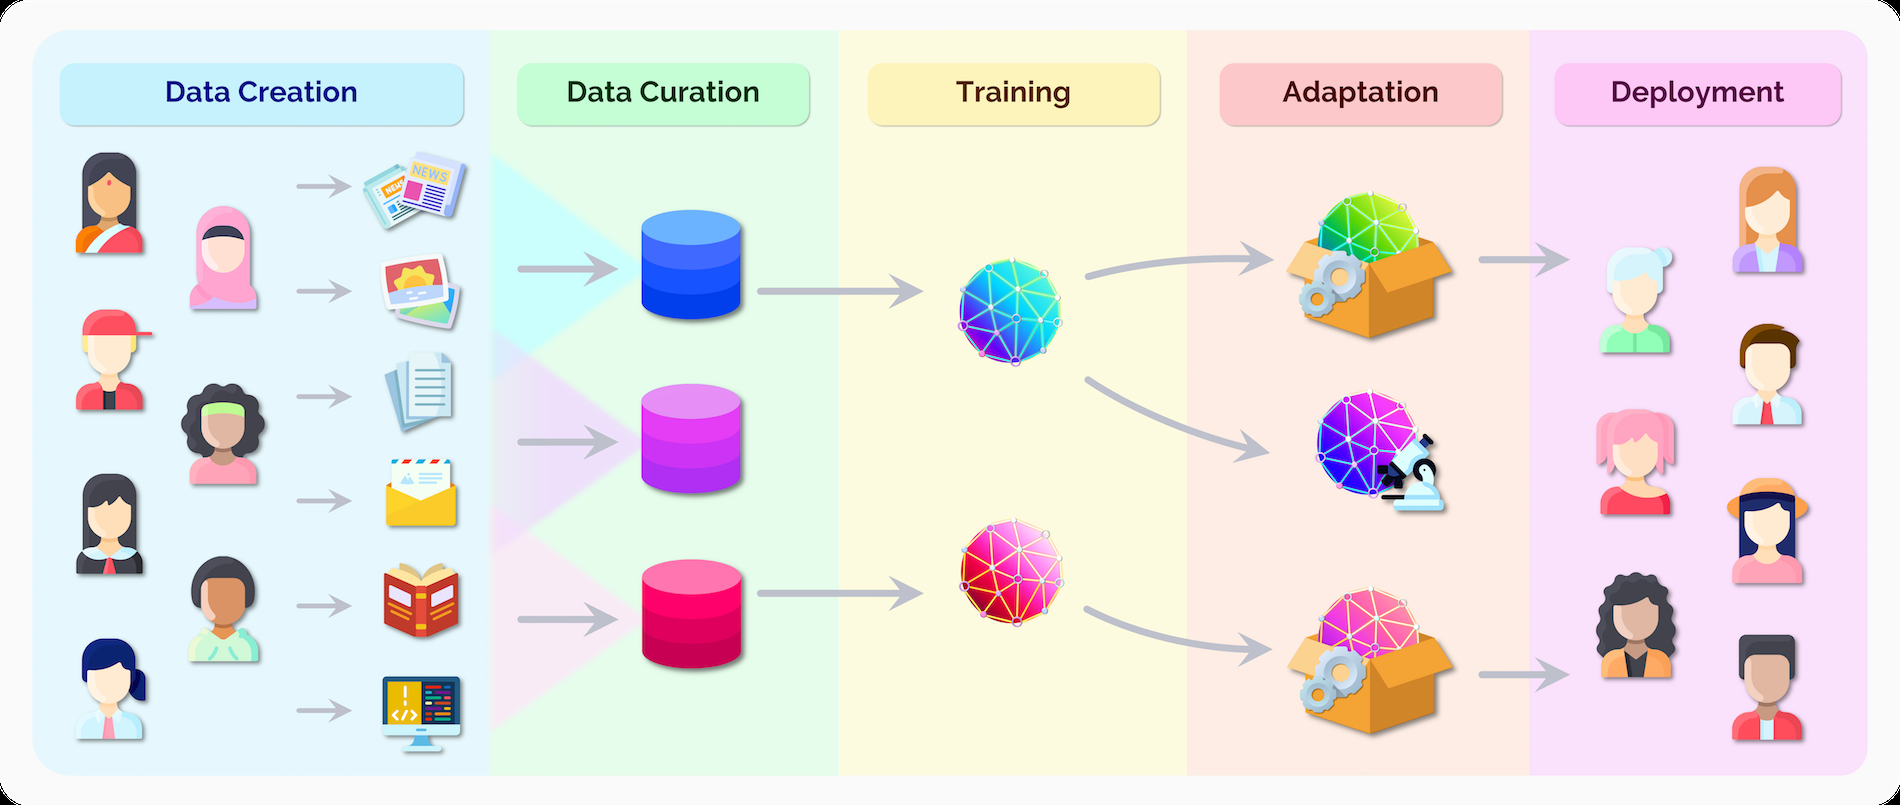
\includegraphics[width=0.5\textwidth]{assets/New-Lecture_Foundation_models/crfm2108_fig3_ecosystem_pipeline.png}\\[0.1em]
  {\scriptsize Fig.~3: From people and data through training and adaptation to deployment (Bommasani et al., arXiv:2108.07258).}
\end{frame}
